\documentclass[../rapport.tex]{subfiles}

\begin{document}

\subsubsection{Diagramme des cas d'utilisation de l'application 1}
Ici il a simplement fallu ajouter 2 utilisations : Afficher l'historique des taux de conversion et calculer un taux de conversion. Nous verrons plus loin que tout est implémenté sur la meme Scene.
\begin{figure}[H]
    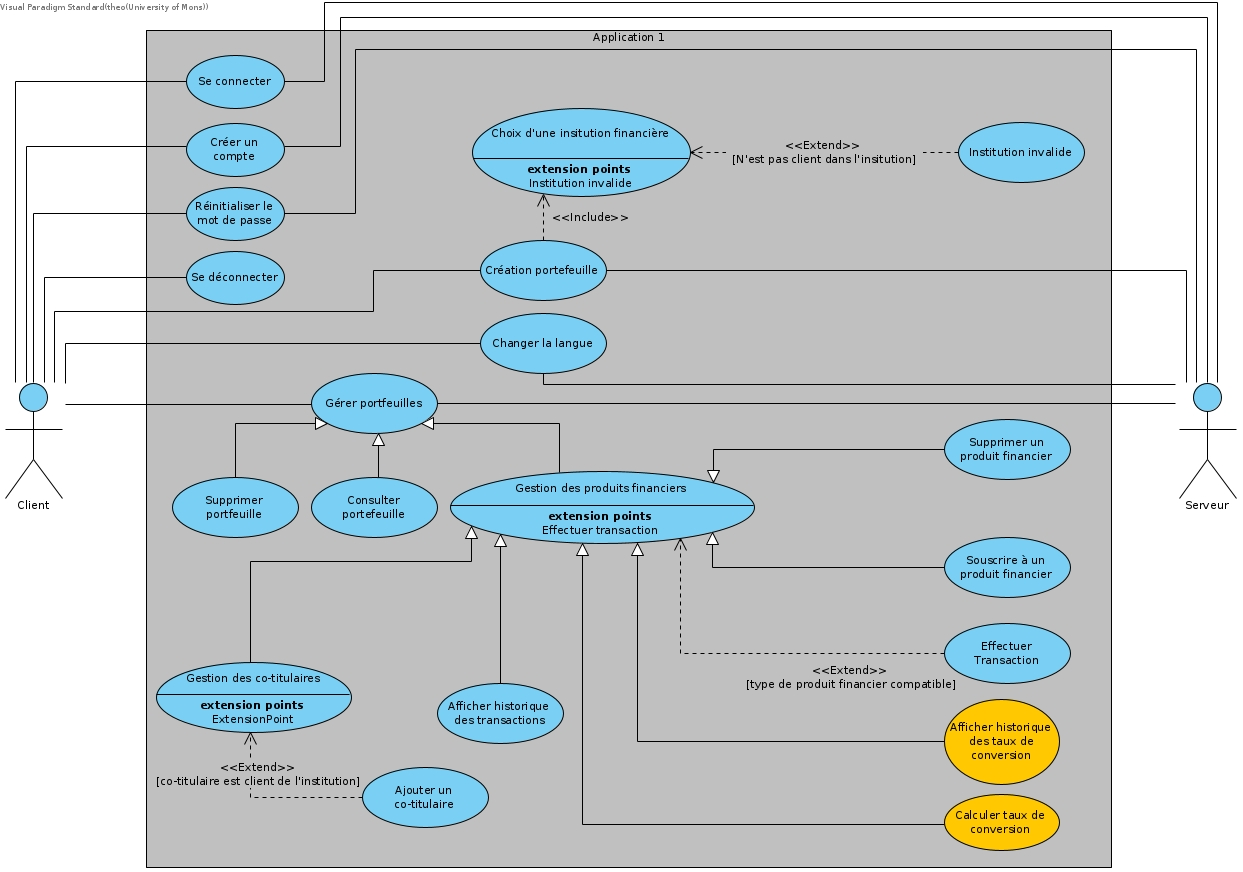
\includegraphics[scale=0.288]{ressources/photos_diagrammes/extensionUgo/useCaseApp1.jpg}
    \caption{}
\end{figure}

\subsubsection{Diagramme de séquence}
Un seul diagramme de séquence est nécessaire, celui ci décrit comment l'utilisateur interagit pour calculer un taux de change. On peut aussi noter l'utilisation d'une API externe (ExchangeRate-API) et d'un parser JSON afin de bien formatter les données.
\begin{figure}[H]
    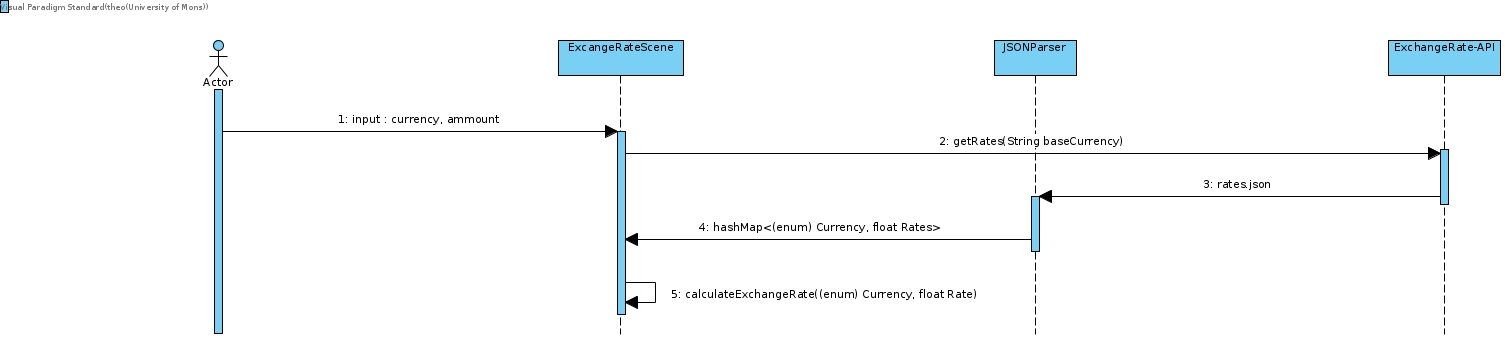
\includegraphics[scale=0.288]{ressources/photos_diagrammes/extensionUgo/calculateExchangeRate.jpg}
\end{figure}

\subsubsection{Classes de l'application 1}
L'ajout d'une fenêtre dans le GUI de l'application 1 implique l'ajout d'une nouvelle classe contenant des variables (qui serviront à stocker les données relatives au taux de change) et une méthode qui servira à afficher le résultat.
\begin{figure}[H]
    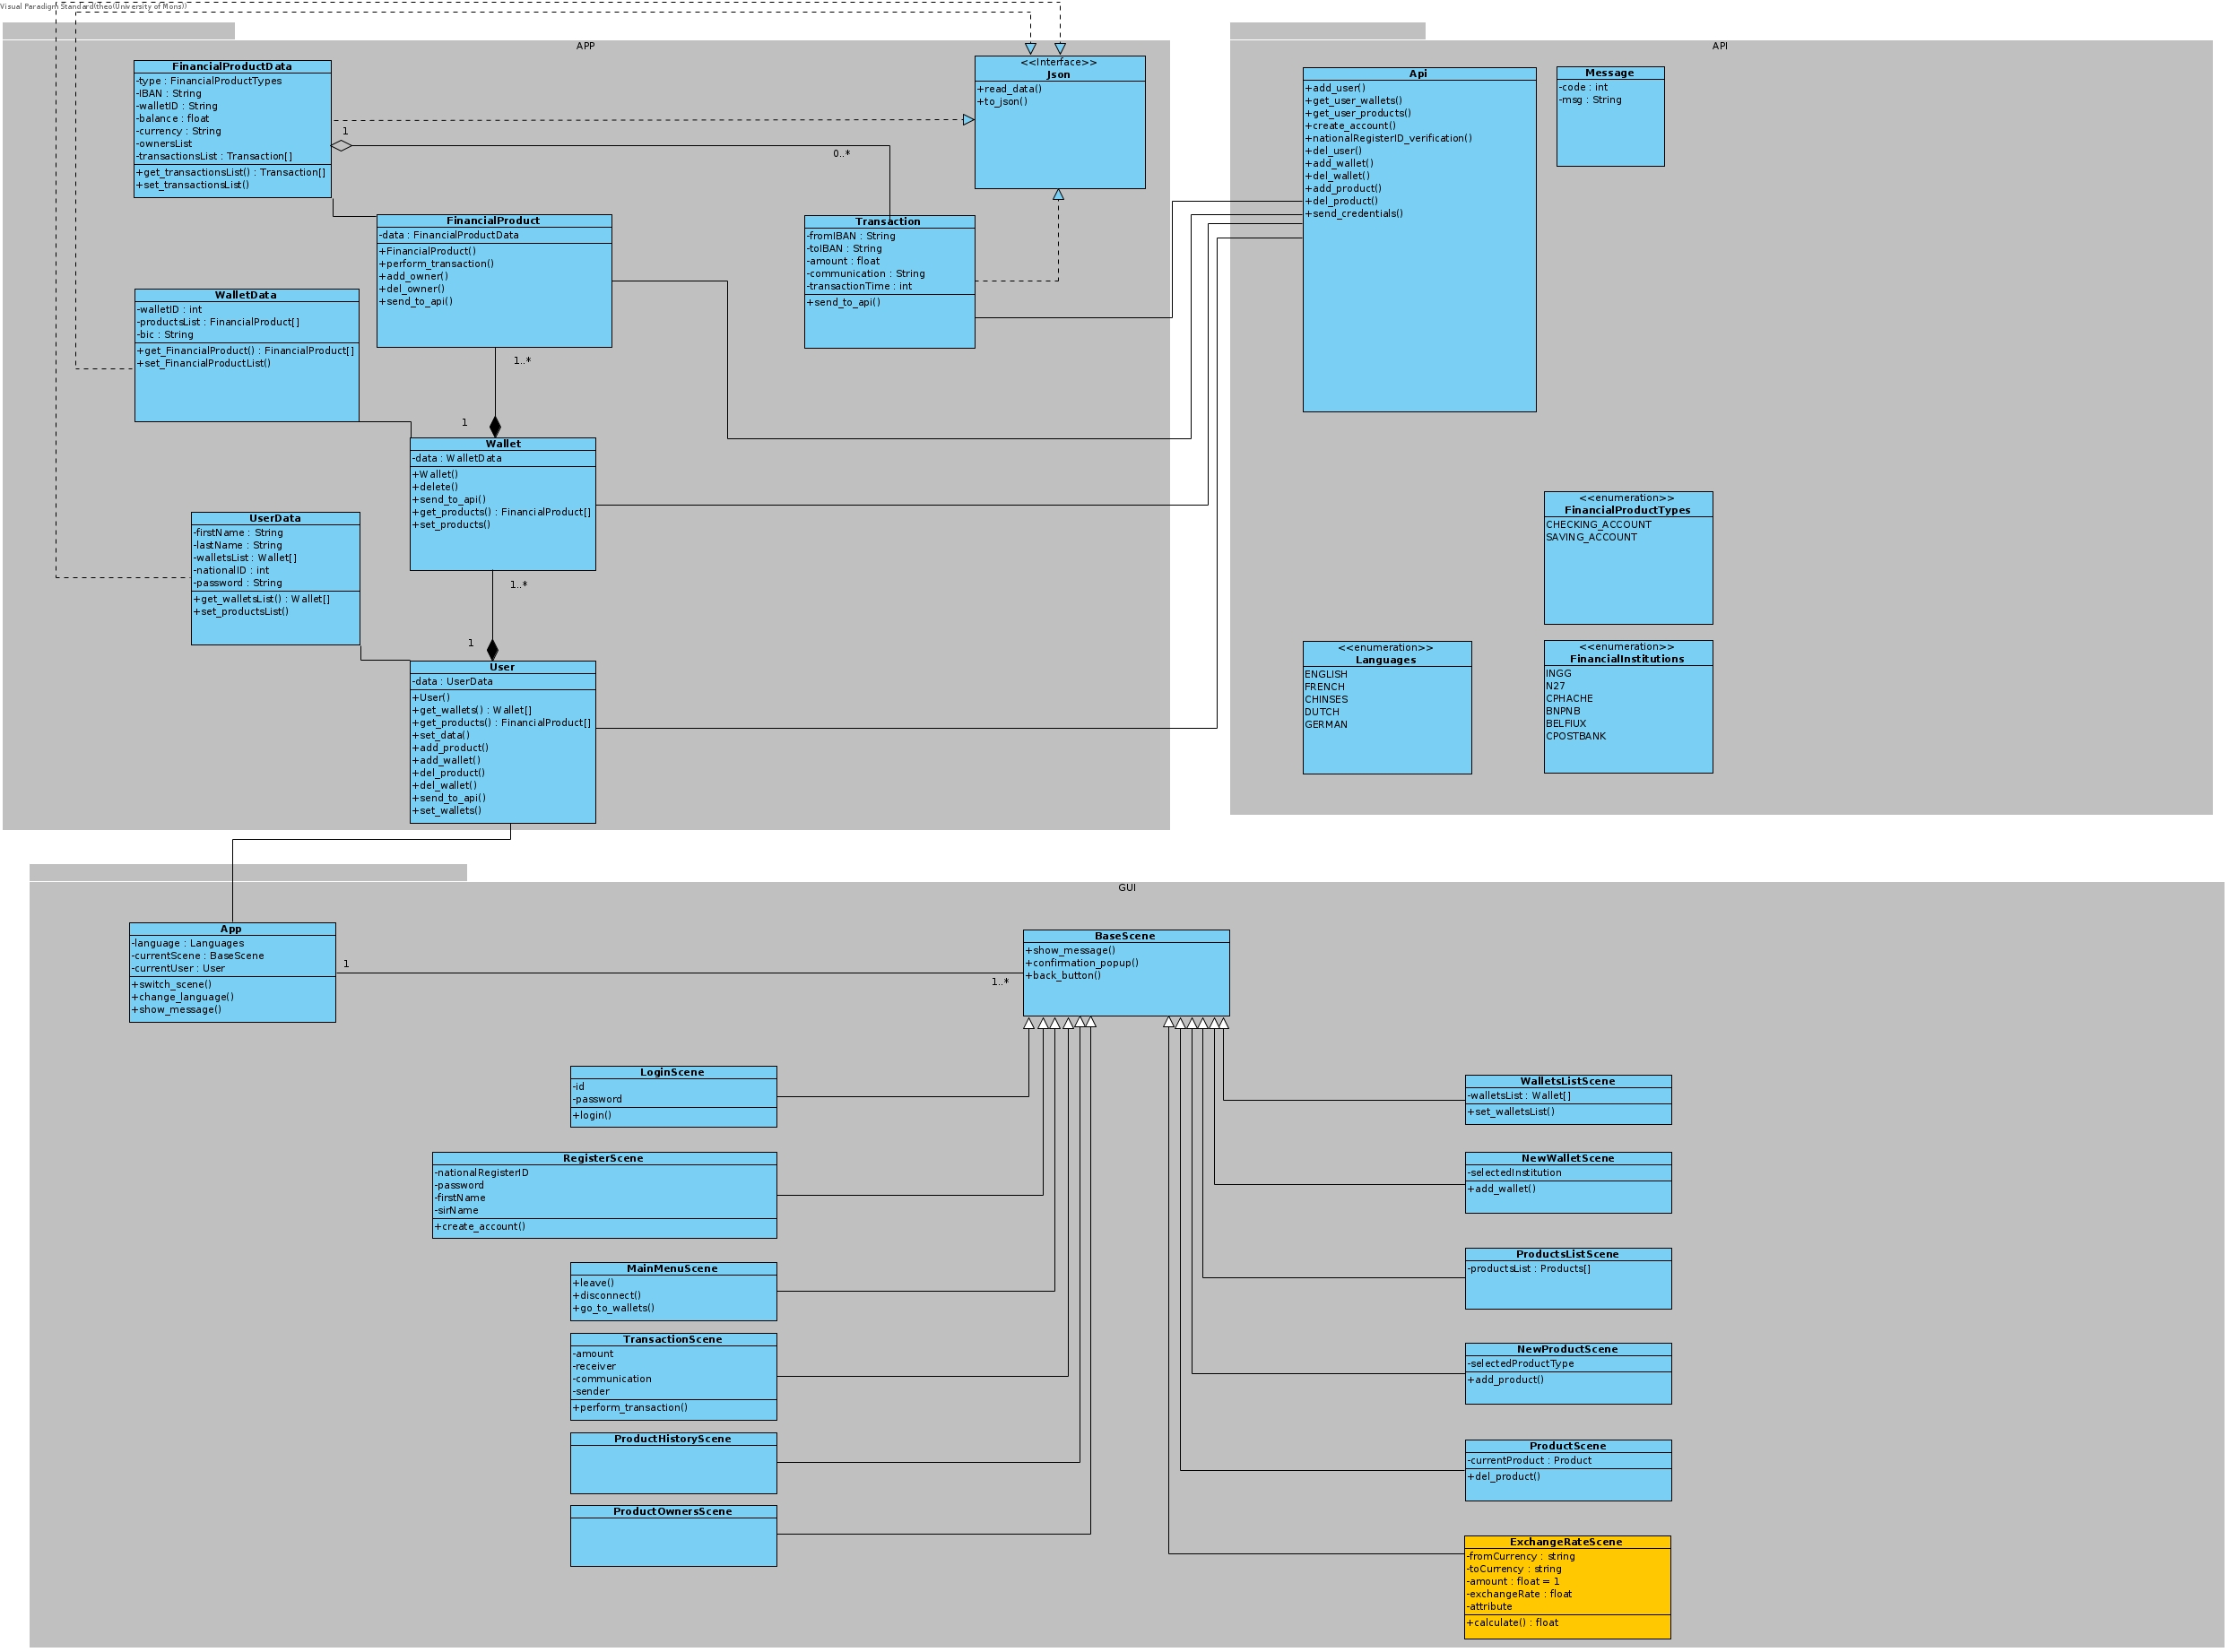
\includegraphics[scale=0.188]{ressources/photos_diagrammes/extensionUgo/classDiagramApp1.jpg}
\end{figure}

\subsubsection{Classes de l'application 2}
L'ajout d'une fenêtre dans le GUI de l'application 2 implique l'ajout d'une nouvelle classe contenant des variables (qui serviront à stocker les données relatives aux frais de transaction) et une méthode qui servira à définir les frais (et les envoyer à l'API).
\begin{figure}[H]
    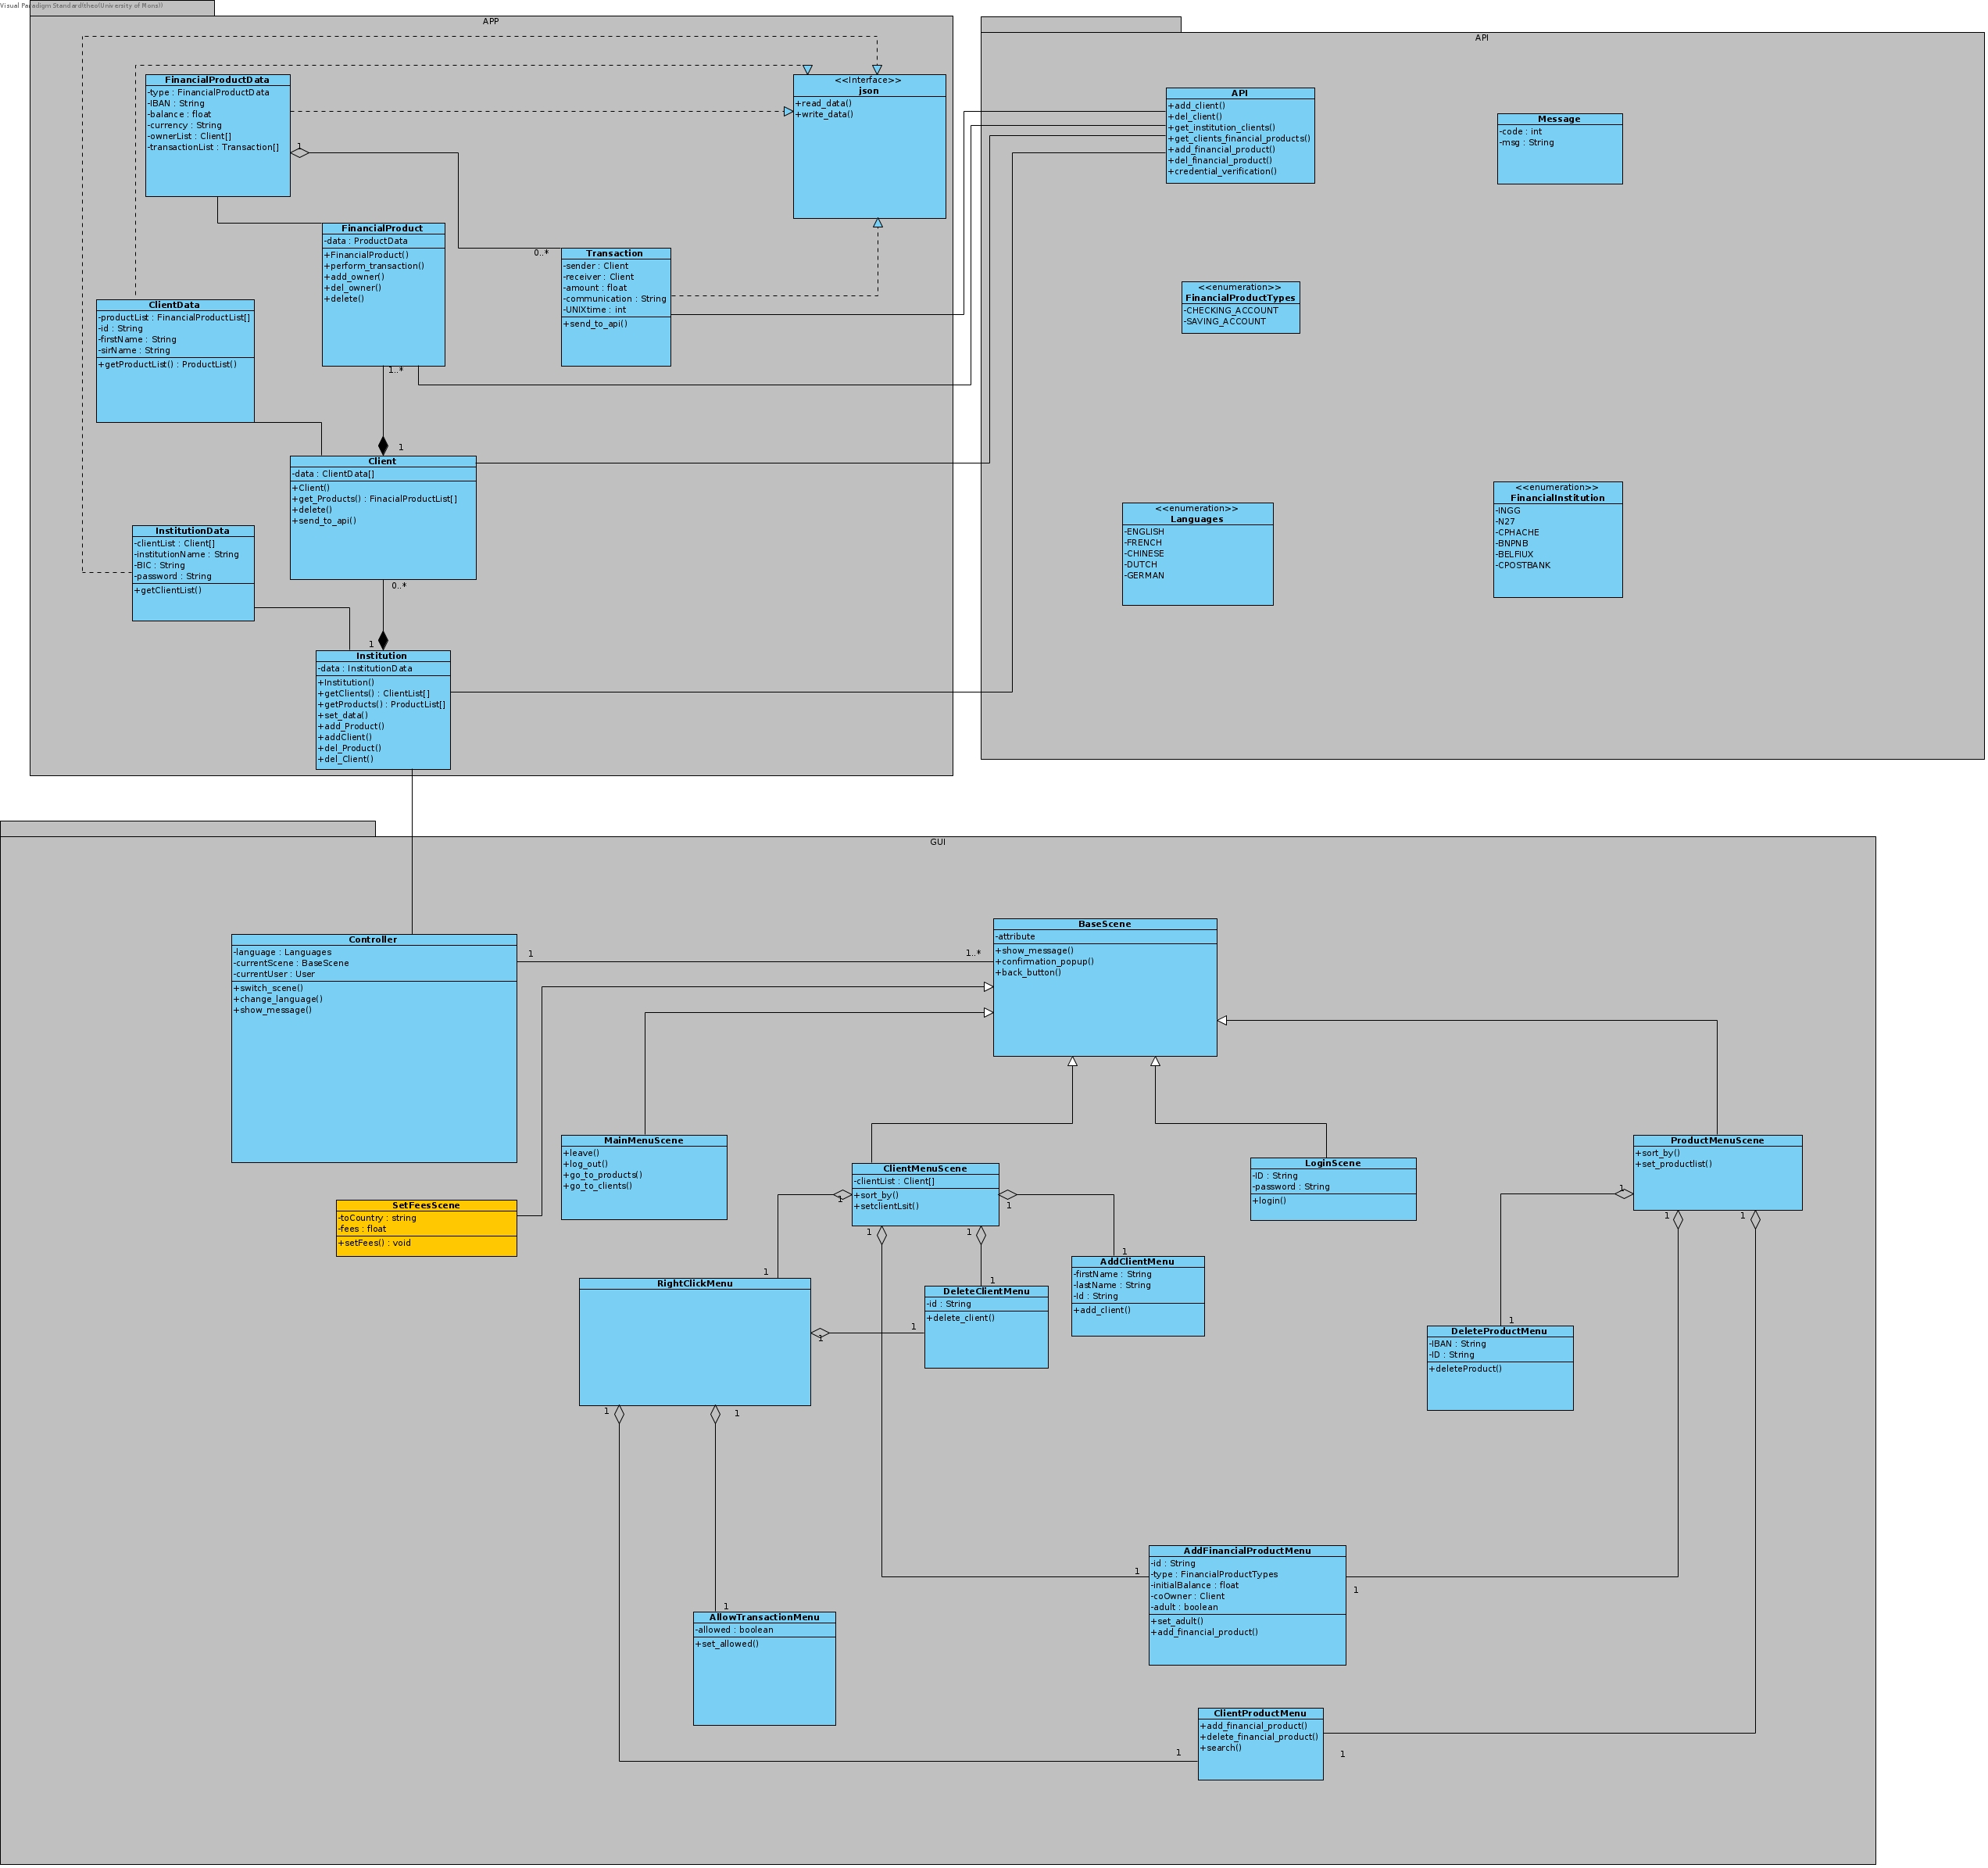
\includegraphics[scale=0.188]{ressources/photos_diagrammes/extensionUgo/classDiagramApp2.jpg}
\end{figure}

\subsubsection{Interface graphique de l'application 1}
Sur cette Scene, l'utilisateur peut introduire une monnaie et un montant (en dessous du texte Base currency), introduire une monnaie destination et voir le taux de change utilisé ainsi que la valeur finale. \\
La partie batch mode est très pratique car elle affiche le taux de change de plusieurs monnaies afin d'avoir une vue globale rapide. \\
Le graphique en bas affiche le taux de change des deux monnaies choisies au dessus dans le temps.
\begin{figure}[H]
    \includegraphics[scale=0.288]{ressources/photos_diagrammes/extensionUgo/ExchangeRateScene.jpg}
\end{figure}

\subsubsection{Interface graphique de l'application 2}
Cette fenêtre est assez simple, l'institution entre un pays de destination ainsi que les frais. Les données sont inscrites dans la base de données et un message (en vert) confirme le changement.
\begin{figure}[H]
    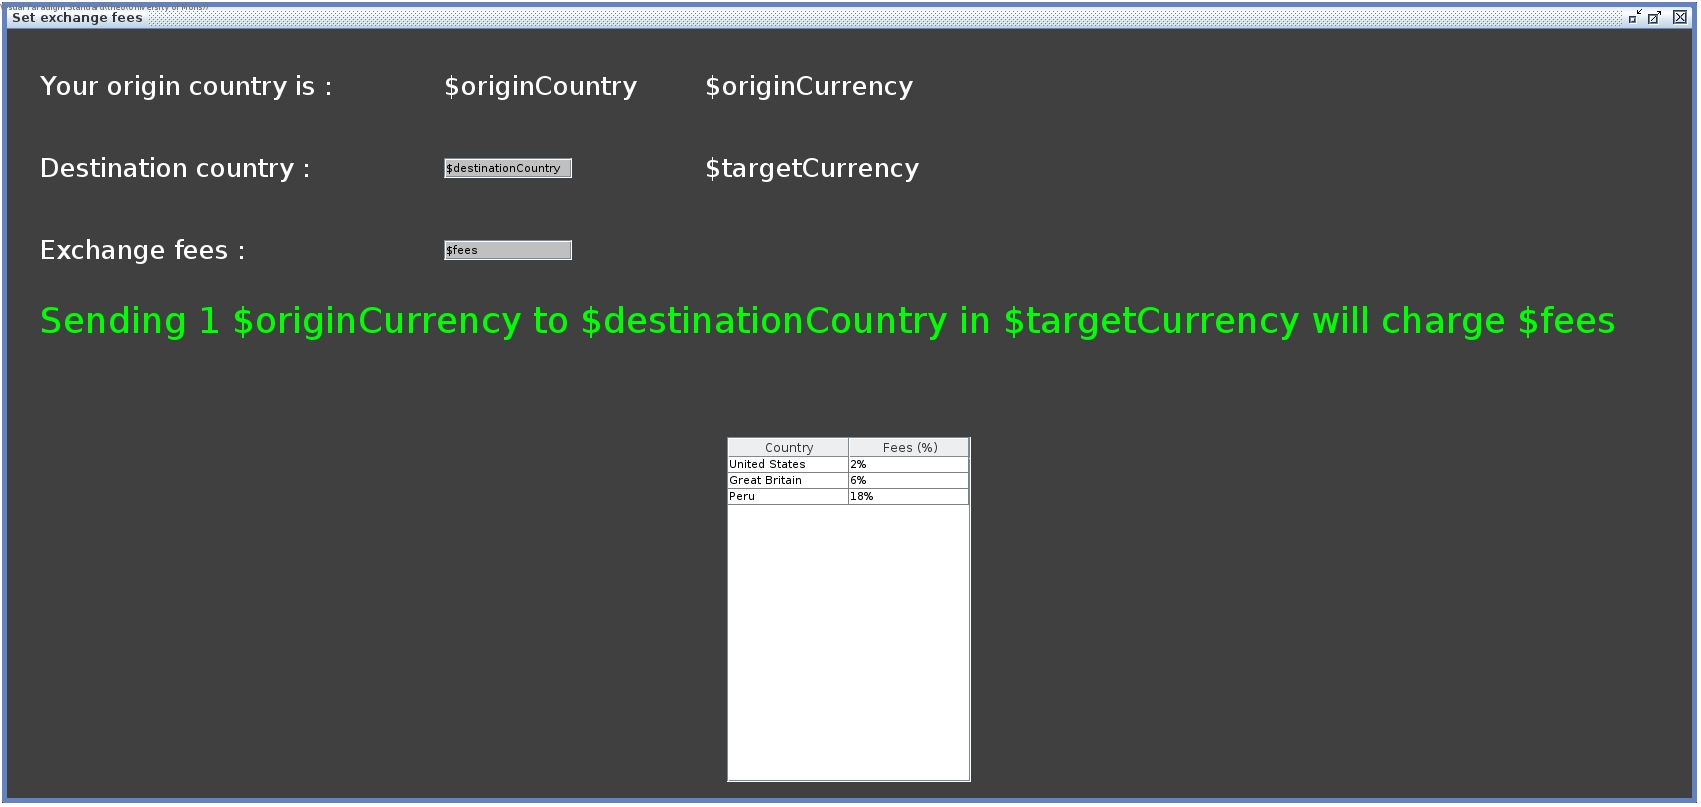
\includegraphics[scale=0.258]{ressources/photos_diagrammes/extensionUgo/setFeesScene.jpg}
\end{figure}

\subsubsection{Diagramme de l'API (financial product)}
Comme expliqué juste avant, une institution doit pouvoir enregistrer dans la base de données des frais de transaction. Il nous faut donc cette fonction dans l'API.
\begin{figure}[H]
    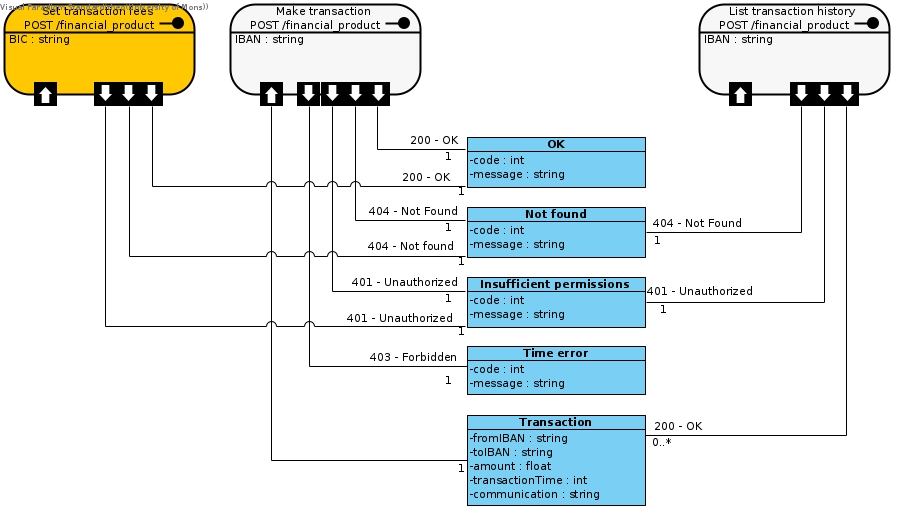
\includegraphics[scale=0.288]{ressources/photos_diagrammes/extensionUgo/financial_productAPI.jpg}
\end{figure}

\subsubsection{Base de données}
Une table permet de stocker les frais de transaction. Une autre pour garder l'historique des taux de change car ExchangeRate-API ne le permet pas.
\begin{figure}[H]
    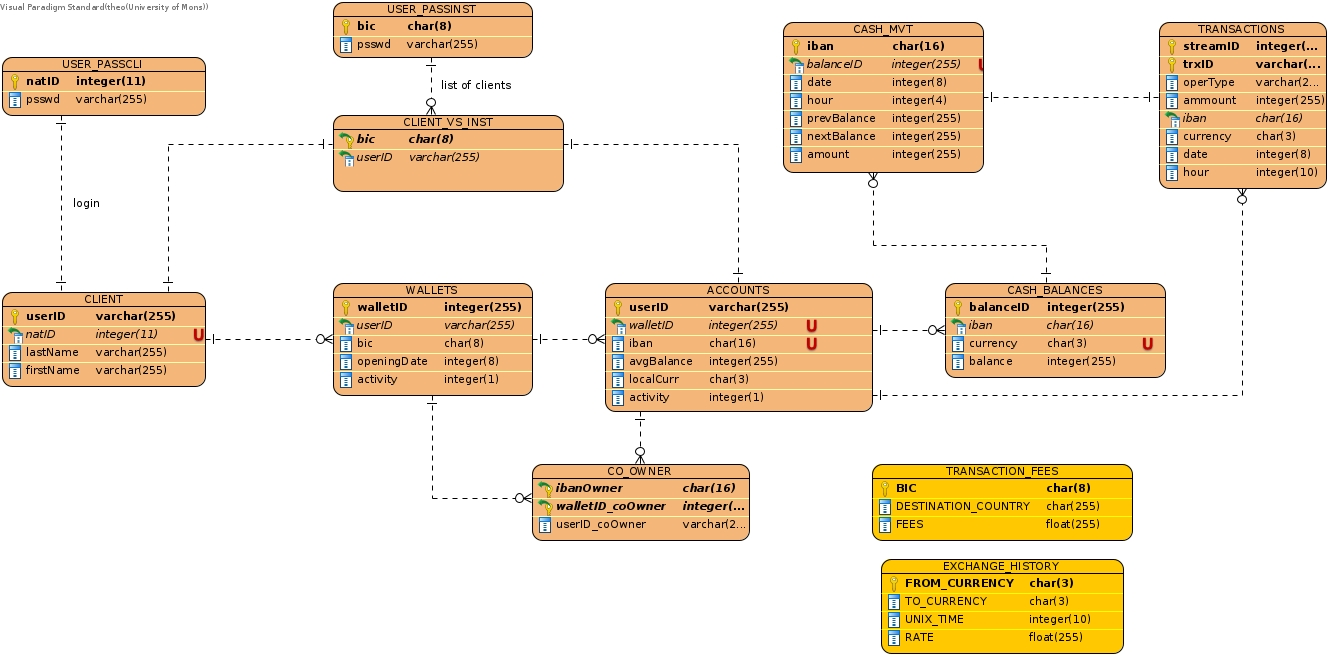
\includegraphics[scale=0.288]{ressources/photos_diagrammes/extensionUgo/ERD.jpg}
\end{figure}

\subsubsection{Interaction Overview Diagram 1}
\begin{figure}[H]
    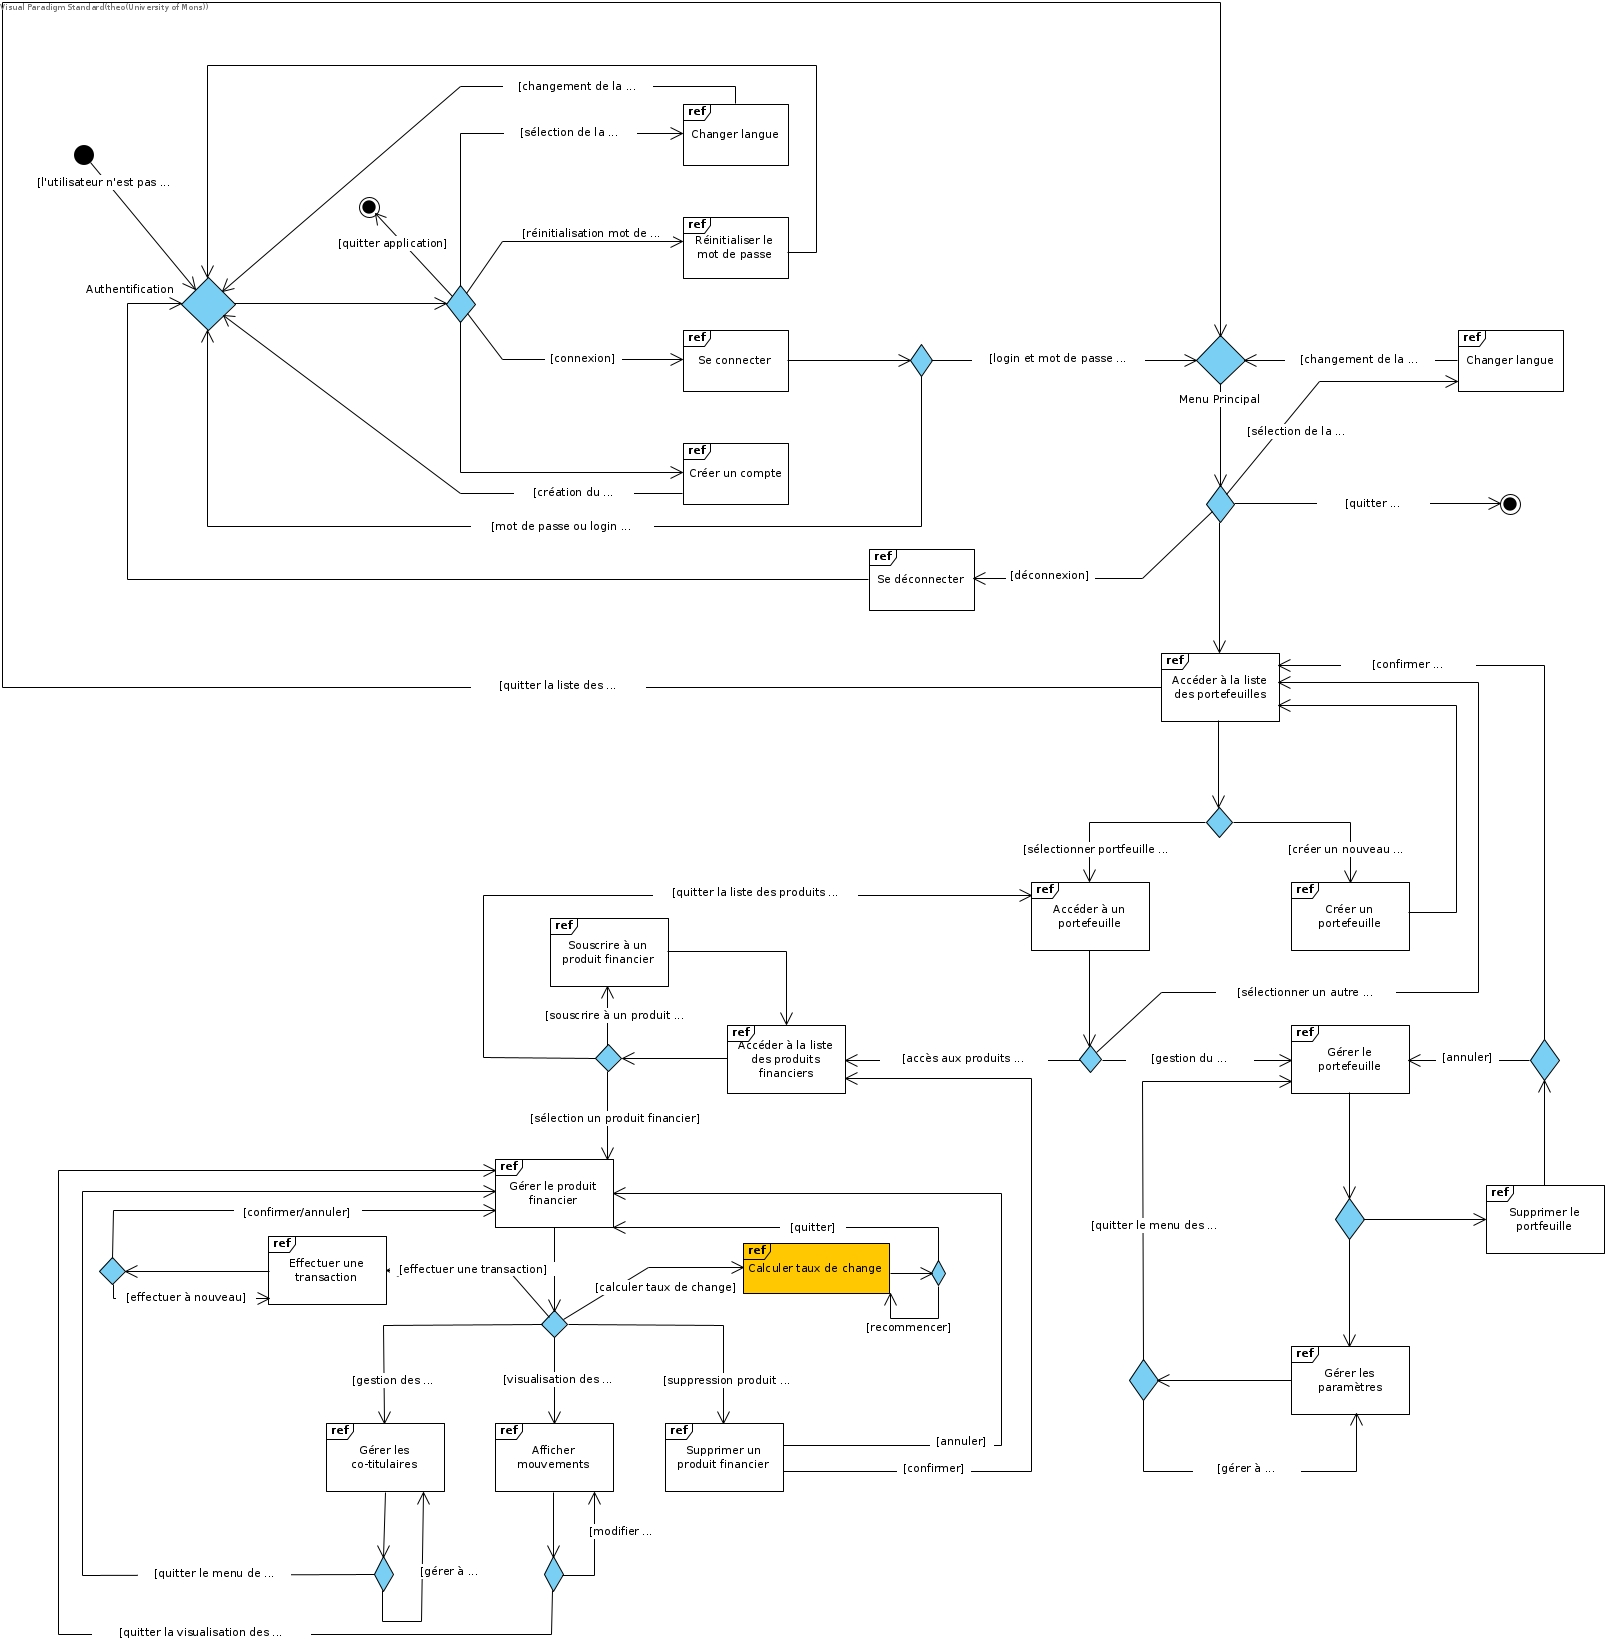
\includegraphics[scale=0.288]{ressources/photos_diagrammes/extensionUgo/interactionOverviewDiagramApp1.jpg}
\end{figure}

\subsubsection{Interaction Overview Diagram 2}
\begin{figure}[H]
    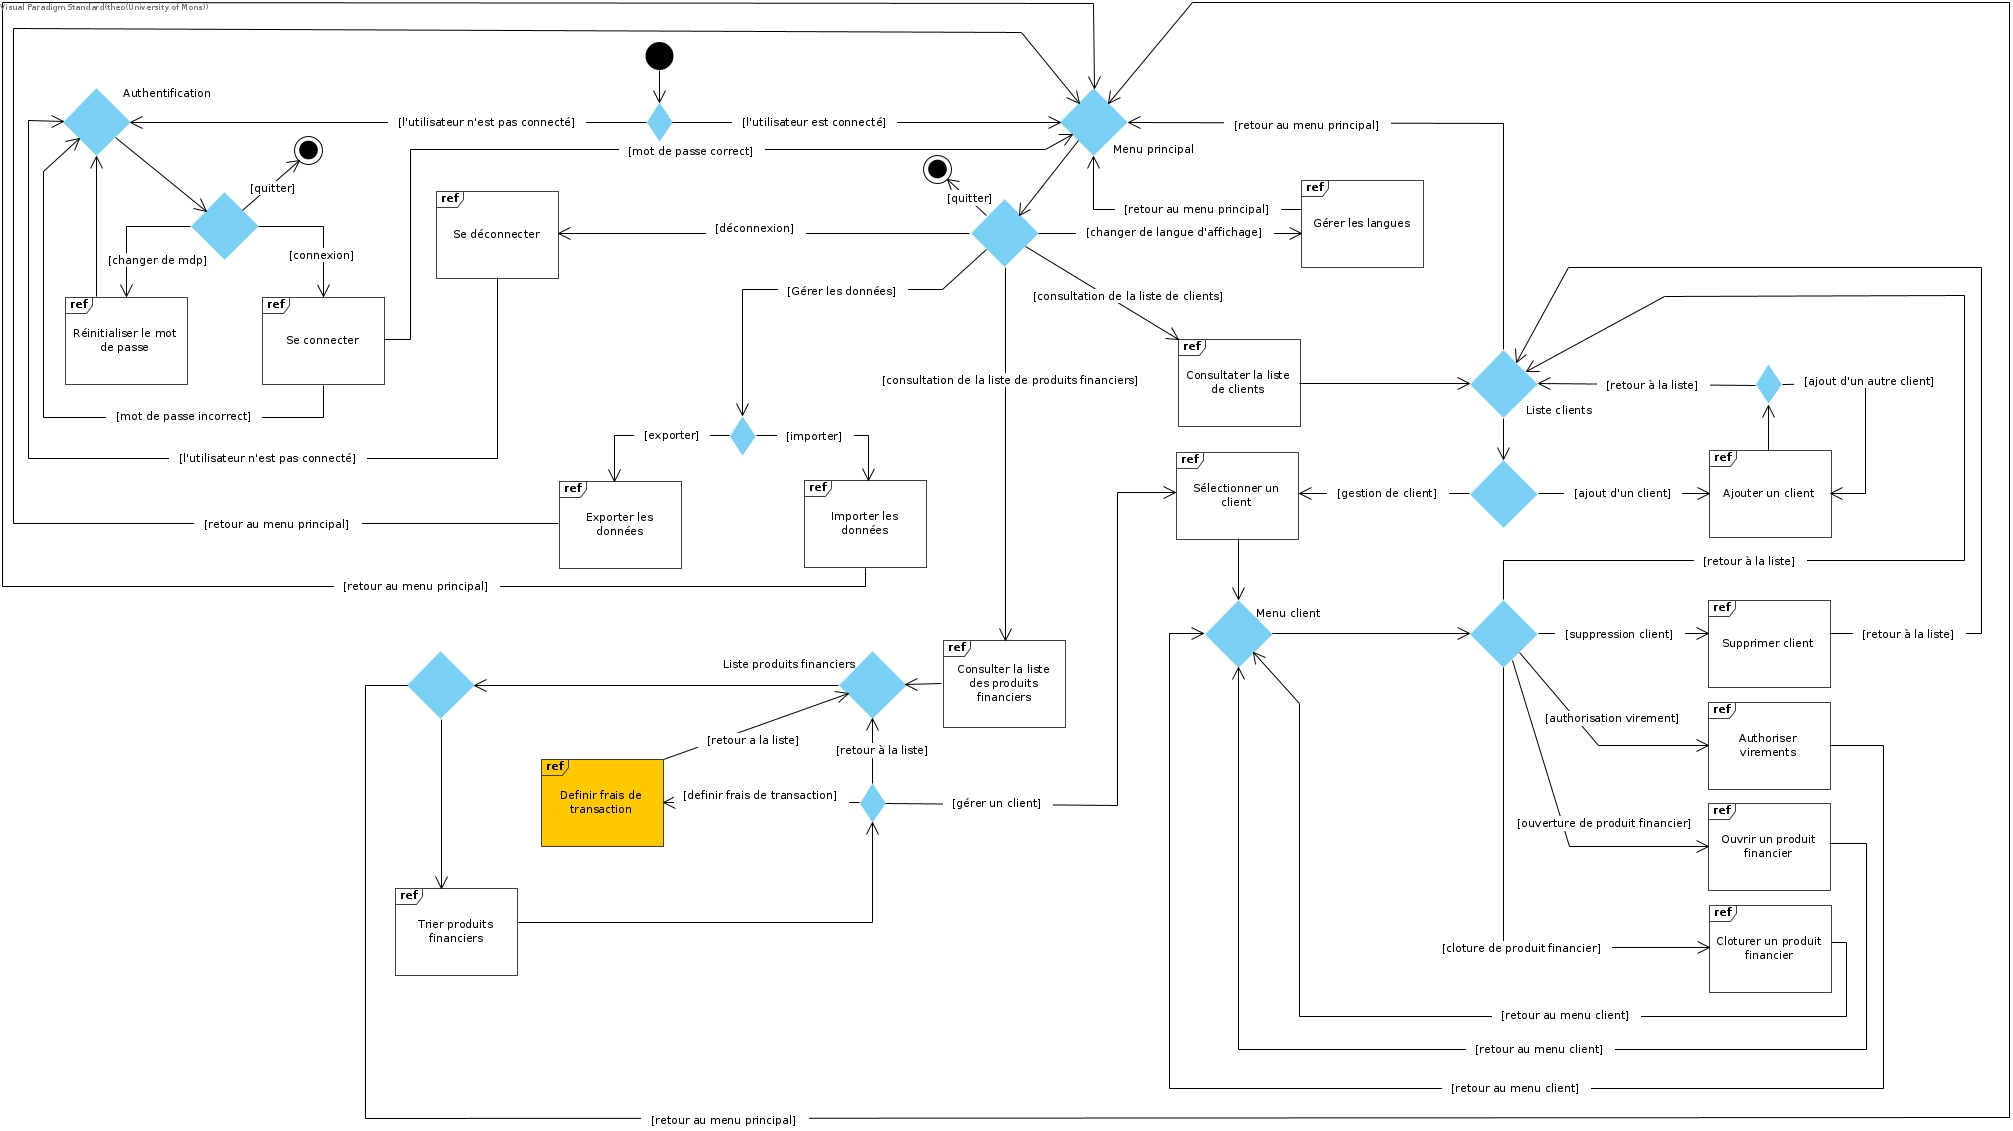
\includegraphics[scale=0.188]{ressources/photos_diagrammes/extensionUgo/interactionOverviewDiagramApp2.jpg}
\end{figure}

\newpage

\end{document}
